%=========================
% Materials and Methods
%=========================
%============NOTE==============
% Check tense !!! It should be present and future tense and mostly passive voice.
%==============================

% 1. Why is this section in past tense? I thought when we talked in my office we agreed, Literature Review refers to work that's been done. Materials and methods refers to work that YOU want to do for your dissertation, which means it's not done yet unless this is your dissertation, in which case it's past tense because you're writing up what you've done for your research.

% Again. This "outline" seems to be a proposal. It should be written in FUTURE tense. You're writing this in a mishmash of present, future and mostly past tense. Save past tense for the dissertation after you've actually done the work.

This research will use data collected from surveys of irrigated lowland rice growing areas in South and South East Asia to examine relationships between the injuries caused by pests and diseases, cropping practices (\textit{e.g.}, rice variety grown, crop establishment method, fertilizer and chemicals applied), and rice yields. Their relationships will be constructed and analyzed through network analysis. I will develop and apply suitable methods of network analysis to characterize the associations of injuries and cropping practices. The resulting network of associations of injuries and cropping practices will thus provide a starting point for further investigations of their relationships (\textit{i.e.}, comparison of networks under different production environments or examination of networks at different levels of yield gains). 

Network analysis of rice crop health survey data is divided into three parts. In the following, I present three distinct network analysis approaches: single-network analysis, differential network analysis, and dynamic network analysis. These three approaches will answer different questions. I will apply single-network analysis to the data from all fields surveyed for identifying patterns of interactions between injuries and cropping practices and key components (\textit{e.g.}, most connected variables). Second, differential network analysis will aim to uncover similarities and differences of networks constructed from the different data sets (\textit{e.g.}, dry season versus wet season). Dynamic network analysis, the third type, will be applied to study how networks changed under at least two different aspects of an evolving complex system. Here, I will focus on dynamic networks by dividing farms into different levels of yield attained. 

\subsection*{Crop health survey data}
\addcontentsline{toc}{chapter}{Crop health survey data}

Crop health survey data were collected through surveys of farmers' fields from 2009 to 2015 for both wet and dry seasons in different production environments across South and South East Asia representing irrigated lowland rice growing areas West Java, Indonesia; Mekong River Delta and Red River Delta, Vietnam; Tamil Nadu and Odisha, India; and Suphanburi, Thailand. The survey protocol described in the IRRI publication, ``A SURVEY PORTFOLIO TO CHARACTERIZE YIELD-REDUCING FACTORS IN RICE'', \shortcite{Savarysurvey2009} was used for data collection. The variables collected included environmental attributes, patterns of cropping practices, crop growth measurement and crop management status assessments, measurements of levels of injuries caused by pests, and direct measurements of actual yields from crop cuts. 

The survey data collected using the methodology described above consisted of measures of multiple variables. These variables can be classified into three groups: cropping practices, injuries, and actual yield measurements. 

Cropping practice data included information on the type of rice variety (traditional variety, modern variety, or hybrid rice), crop establishment methods used (direct seeded or transplanted rice) were collected as categorical data, pesticide usage (molluscicide, herbicide, insecticide and fungicide) were collected as discretized data, and accumulated organic, synthetic fertilizers were collected as continuous data.

% I uncommented and edited this, this is important information, I think.
Injury data were gathered on diseases, insects and weeds observed at two development stages of the growing crop: active tillering and active ripening. While injuries due to diseases and insects were specific to species (or species groups), information on weed infestation was the area covered by any weed species, either above or below the crop canopy. Information pertaining to injuries was collected in the form of number of injured organs (tillers, leaves, and panicles), which later was made relative to the corresponding total number of organs present in the sampling units; 12 hills per field for transplanted rice crops, or 12 10 $\times$ 10 cm quadrat for direct seeded rice. As for weed infestation, the proportion of soil area covered at two levels of the crop canopy (below or above it) was assessed in three points in the field of 1 $mathrm{m}^{2}$ each. For this purpose, two types of injury indices were used: area under injury progress curves (AUIPC) or maximum level at any of the two observations, depending on the nature of the injury. Injuries which is occurred on tillers, hills and panicles will be collected maximum level, whereas juries which are occurred on leave will be collected AUIPC. The area under injury progress curve (AUIPC) was calculated by the mid- point method using the following equation: $\mathrm{AUIPC} = \sum{x\to\infty}\frac{1}{(x_{i} + x_{i-1})(T_{i} - T_{i-1})}$, where $x_i$ is percentage (\%) of leaves, tillers or panicles injured caused by pests (e.g., leaf blast, leaf folder), percentage (\%) of weed infestation (ground coverage) at the \textit{i}th observation, $\mathrm{T}_{i}$ is time in rice development stage units (dsu) on a 0 to 100 scale (10: seedling, 20: tillering, 30: stem elongation, 40: booting, 50: heading, 60: flowering, 70: milk, 80: dough, 90: ripening, 100: fully mature) at the \textit{i}th observation and n is total number of observations.

% Insert a short para describing the crop cutting and weight measurements here, please. Sith: I would not like to include in here because during phase one one protocol and phase two there are some modification in the protocols.

Yield data will be measured from each of the fields, three crop cut 5 $\mathrm{m}^{2}$ (2 $\times$ 2.5 meters), desperately harvested, dried to 14\% moisture content, and separately weighted. The three harvest areas should be taken at random over the field areas. 

\section*{Single network analysis of crop health survey data}
\addcontentsline{toc}{chapter}{Single network analysis of crop health survey data}
\textbf{Introduction}

% Last sentence is unclear, clarify please
Single-network analysis is used for analyzing a network based on a single data set. It aims to model patterns of relationships between entities to a network, thereby determining its topological properties such as node degree, degree distribution, average path length, clustering coefficient, modularity index \shortcite{newman2006modularity} to describe the patterns in the network model. These structural properties offer the potential to explore relationships within complex data sets and identify key factors or clusters.

% These are only used for biological systems?
Correlation based networks are widely used for studying biological networks based on pair--wise correlations between variables. Their edges are obtained using correlation-based measures removing spurious relationships. Correlation based measures include linear based correlation (Pearson's correlation, partial correlation) and rank based correlation (Spearman's correlation, Kendall's correlation). Removal of spurious relationships is particularly important when one attempts to establish causal relationships between entities \shortcite{Toubiana:2013cv}. a correlation based network allows one to define modules (clusters), intramodular hubs, and network nodes with regard to module membership, to study the relationships between modules, and to compare the network topology of different networks (differential network analysis). 

In the case of single network analysis, a network model of cropping practices and injury profiles based on whole data set of surveys will be defined using a correlation as an undirected, weighted network. Nodes of the network corresponded to variables and edges between variables will be determined by their pair--wise correlation. A network model based on crop health survey data has not yet been reported. Additionally, network analysis of these data has not been studied. Thus, correlation measures and network approaches should be evaluated.

% what's the problem of multiple testing? Unclear.
According to \shortciteA{kolaczyk2014statistical}, correlation based network construction has at least three important issues to be dealt with. First, there is the choice of pair--wise correlation measure to be used. Second, the level of statistical significance must be determined for removal of sparse relationships. Finally, the problem of multiple testing must be considered because large numbers of tests for pair-wise comparison lead to increase false discovery rate.

The use of crop health survey data to construct correlation network and perform network decomposition and network analysis has not yet been reported. Additionally, methods performing network analysis and correlation networks has not been studied. Thus, evaluation of such methods is challenging because there are many types of variables mixed in crop health survey data; methods can identify variables with true concordance often determine the prior knowledge; and methods performing biologically meaningful corrleation network construction. 

\subsection*{Single network analysis network construction}

%% 1. First sentence is unclear.
Cropping practices and injury profiles network are constructed from an adjacency matrix originating from the pair--wise correlations of the incidence of injuries (insect injuries and diseases), amount of fertilizer, the frequency of pesticide applied, type of rice varieties and crop establishment methods across different samples. Therefore, edges of the network correspond to the degree of correlation between two variables. A standard measurement of correlation between two variable $x$ and $y$, $cor(x,y)$, where values are  between -1 to +1 depending on the level of relationship. $cor(x_{i}, x_{j})$ is equal to -1 when there is a decreasing relationship between $x$ and $y$, and +1 when there is a increasing relationship.

To identify the most suitable pairwise correlation methods, I will evaluate four correlation based measures, Pearson's correlation, Spearman's rank correlation, Kendall's correlation, and biweight midcorrealtion. R was employed to compute pairwise correlation \shortcite{R:2014a}. The \texttt{cor.test()} function will be applied for generating a correlation matrix, which describes the pairwise correlations between variables. This function allows users to choose types of correlation measures to perform such as Pearson's correlation, Spearman's rank correlation and Kendall's rank correlation. To compute biweight midcorrelation, I will apply the \texttt{bicor()} function from the \textbf{WGCNA} package \shortcite{Langfelder:2008bd} in R. 

% 1. Why would p-values be concerned? They aren't capable of being concerned. People can be concerned, p-values are not people.
% 2. I don't understand your last sentence here?
When a correlation matrix is created, next is to construct the correlation based network. However, $p$~values should be determined. As with issues previously mentioned above, $p$~values must be adjusted for multiple testing. Using a Benjamini-Hochberg adjustment or Bonferonni correction is recommended by \shortciteA{kolaczyk2014statistical}.  The \texttt{fdrtool()} function of \textbf{fdrtool} R package can calculate adjusted $p$~values. These values are compared to a standard 0.05 significance level. The final correlation matrix contains pair-wise correlation coefficients, which have adjusted for $p$~values lower than 0.05 significance level. 

% 1. The first sentence after that is still unclear.
R packages: \textbf{igraph} \shortcite{Csardi:2010wx}; \textbf{qgraph} \shortcite{qgraph}; \textbf{statnet} \shortcite{statnetpackage} and \textbf{network} \shortcite{networkpackage}; and \textbf{sna} \shortcite{snapackage} will be applied to construct network models from four association metrics; Pearson coefficient, Spearman coefficient, Kendall coefficient and Biweight midcorrelation, to decorate the network, and then analyze the network structure.

%% 1. Second sentence. Clarity/grammar (affect to?)
A network modeled from biological data may not reveal useful biological information, even though it is created from a method based on its principle of statistical operation \shortcite{evaluationKumari}. For correlation based networks edges correspond to correlation coefficients and also affect to the network structure and behaviors. Different correlation based measures contribute to networks with different structures, even though they are constructed from the same data set. I will investigate the efficiency of networks based on four correlation measures for revealing the associations between variables of surveys. The most suitable correlation measure is assumed that it can contribute the network being able to reveal the associations between variables based on the existing literatures or good understandings of biological relationships between variables that crop health surveys observed.

%====================== Comments===================
% why knowledge of biological literature? Why not a good understanding of the biological system that you are monitoring? I think that's more essential and useful
% models cannot reveal knowledge, look up the definition of knowledge. It does not apply here. What do you really mean because it can not be knowledge?
% first sentence, all of them what?
% based on what study? Our study? Who is "we"? This is YOUR research. If anything it should be "based on my study" but I'm not clear as to what study you refer to here. Who are the "we" that are suggesting? You're the only author on this manuscript. It's your dissertation. There is no, our, us or we. It's only my, me, I here.
% Is "codes" the proper form to use?

\subsection*{Evaluating network properties}
% You have already cited qgraph and igraph, it's not necessary to again, I don't think, in the same way that you don't constantly keep citing R every time you mention it after you cited it the first time.
% I'm not even sure what this sentence is: " I particularly are interested in properties potentially relevant for biological roles and functioning as previously hypothesized in other biological networks \shortcite{Strogatz:2001wc, qgraph, horvath2011weighted}." Please revise for clarity and grammar.
Once a network is constructed several indices can be computed to convey information about network structure. To evaluate the topological properties of both the interaction and the correlation based network, I will use the packages \textbf{igraph} and \textbf{qgraph} in R. I particularly are interested in properties potentially relevant for biological roles and functioning as previously hypothesized in other biological networks \shortcite{Strogatz:2001wc, qgraph, horvath2011weighted}.

% what is this section? You need some sort of introduction to this list of items.
\begin{enumerate}
\item Mean degree: the degree of a node counts the number of edges it has. The mean degree is calculated over all nodes in the network.
\item Degree distribution: the frequency of nodes vs. their (increasing) degree.
\item Average shortest path length: the shortest path between any two nodes is the single path with fewest edges between them. Alternative paths are feasible. The average shortest path length is the mean over all shortest paths between any two nodes in the network.
\item Mean clustering coefficient: a cluster of nodes is a triangle of nodes. The clustering coefficient calculates the fraction of observed vs. possible triangles for each node. The mean is subsequently determined from all nodes in the network.
\item Betweenness centrality: the betweenness centrality of a node is equal to the number of shortest paths between any two nodes in the graph passing through that node. The mean is calculated from all nodes in the network.
\item Closeness centrality: the closeness centrality of a node is given by the average distance of this node to any other node. Again, the network-wide measure is an average over all nodes in the network.
\end{enumerate}

\shortciteA{Deng:2012do, Toubiana:2013cv, horvath2011weighted, newman2003structure} are recommended references for descriptions of the network properties as well as the formal calculation of these measures.

%====================================================
\section*{Differential network analysis of crop heath survey data under different seasons and production environments}

% Should this analysis include more than one season or production environment since you say it's differential? Your section header above would indicate this to be true.

\addcontentsline{toc}{chapter}{Differential network analysis of crop health survey data under different season and production environment}

% Recheck this para. It's not clear to me what it's saying. I've tried to help, but am still not sure.
Networks can respond differently under various environments or with external signals.

They can be simplified by focusing on key components and capture only the essential components differently responding between environments which they play a key role in the modeled response \shortcite{Peer:2011jd}. Networks are examined by adding or deleting some variables. This allows predicting interactions or components that change following the changed structure of networks. 

% 1. This para is difficult to understand. Revise.
% 2. This sentence in particular is unclear:  "Conversely, the interactions are weak or removed from the differential network."
% 3. This sentence is unclear as well: "If networks constructed from different environment conditions, the differential interactions between two networks are implied changes that they are a result of response to environmental conditions."

Differential network analysis is applied to identify and describe differences between two networks under different conditions. Differential networks from different data sets with different conditions might display different interactions from the single network based on the whole data set, which are disregarded the conditions. The strongest interactions in differential networks are not necessarily those that are strong in the single network. Conversely, they may be weak or absent in single network. Compared between differential networks under different environment conditions, the differential interactions can be implied that they are a result of response to environmental conditions. Moreover, it can be implied that environments influence on the interaction between pairs of nodes contributing to the differential interactions. 

% objective
% This para is much improved! It still needs some work to clearly explain your point.
The objective of differential network analysis is to extract interactions from the original network that appear to be active under different conditions. I focus on two aspects of this analysis. The first is to compare how patterns of interactions of cropping practices and injury profile network change across multiple production environments. The second is to study how networks change with different cropping seasons (wet or dry). Each data set is used to construct the network. Next, these networks are contrasted to find a) non-preserved modules, b) differentially occurred variables, and c) differentially connected variables.

% methods
% 1. First sentence is awkward.
Differential networks will be constructed from the survey data with different groups of samples following the purpose of network construction. To analyze differential networks under different seasons, I will construct two networks; one will be constructed from dry season data, and another will be constructed from wet season data. Additionally I will determine differential networks under different production environments (locations).

% 1. You applied the package or a function from a package? # I do not know excactly what function I will use, so I stated the packages that I will use instead of functions of those packages. # OK, noted.
For comparison with a standard differential network analysis, I applied \textbf{WGCNA} \shortcite{horvath2011weighted} and \textbf{dna} \shortcite{dnapackage} package in R, which this package provide several function to analyze the differences of topologies of two networks \shortcite{horvath2011weighted}. 

These packages include preprocessing tools for simultaneously preparing a pair of networks for analysis, procedures for computing connectivity scores between pairs of variables based on many available statistical techniques, and tools for handling modules of variables based on these scores. Also, procedures are provided for performing permutation tests based on these scores to determine if the connectivity of variables differs between the two networks, to determine if the connectivity of a particular set of important variables differs between the two networks, and to determine if the overall module structure differs between the two networks. Several built-in options are available for the types of scores and distances used in the testing procedures, and additionally, the procedures provide flexible methods that allow the user to define custom scores and distances. For example, the \texttt{test.modular.structure()} function is used to compare between the connectivity measures of each network \shortcite{dnapackage}. 

%I propose the overview of differential networks are illustrated in Figure \ref{fig:wholenet}.


% why is 2.3 not 2.1? % The problem there is that you must put the label after a caption, so the label can reference to the figure (it references to the caption, actually). See here: http://www.latex-community.org/forum/viewtopic.php?t=3659 I've corrected this. - ahs
 

\section*{Dynamic network analysis of crop health survey data}
\addcontentsline{toc}{chapter}{Dynamic network analysis of crop health survey data} 

% introduction
% 1. First sentence, unclear, revise.
% 2. Sentence that starts, "It seems clear" is unclear. Revise.
% 3. Revise last sentence for flow.

Biological systems are highly dynamic. They must continuously respond to external signals or the internal state of the system. The responses can be altered slowly or quickly over time \shortcite{Peer:2011jd}. 
Thus, realistically the corresponding biological networks evolve as well.  It seems clear that if dynamic networks enable us to see and understand the systems on how their dynamic effects are changed over time. Some understandings previously have been obtained from studies of dynamics of large networks, for example, gene expression or metabolic fluxes network \shortcite{Idekerdiffnet}.
 
% 1. Revise first sentence for flow.
% 2. Second sentence. Revise for spelling and clarity.
% 2. Third sentence. Revise for spelling and clarity.
Dynamic network analysis will be applied to study changes in networks with at least two different aspects of an evolving complex system. 

The main goal of dynamic network analysis moves away from single network analysis, which characterizes absolute properties of the system. It aims to concentrate on a specific dynamic response. Rather than answer what the key factors in the system, it answers what parts of the system are most affected by perturbation. Most commonly, dynamic networks are applied when the edges among a set of vertices or the sets of vertices itself are changing as a function of time. However, in the context of crop health surveys, I will apply dynamic networks to capture the yield-varying behaviors through different survey data sets grouped by different levels of yield measurements.

% 1. Estimated yields? Crop cuts are not an estimate. They are a direct measurement.
My objectives are to construct and analyze networks of crop health survey data at different levels of farmers' yields. Surveys contain records of observed actual yields, various types of injuries and cropping practices. To generate the data set for constructing the dynamic network, I will group the data with successive levels of yields to obtain different yield data sets in order to construct a dynamic network of yield-varying behaviors. I then will employ \textbf{networkDynamic} \shortcite{networkdynamicpackage} and \textbf{ndtv} \shortcite{ndtvpackage} packages to generate yield-varying networks. The dynamic graphs will be characterized following \shortcite{bilgin2006dynamic, kolaczyk2014statistical}. From the network based perspectives, the results will show the patterns of interactions between nodes how they changed when levels of yield decreased or increased.


% I think your figures are useful. Why are they commented out? Please reinsert them before this is submitted.

%\begin{landscape}

\begin{figure}
\centering
%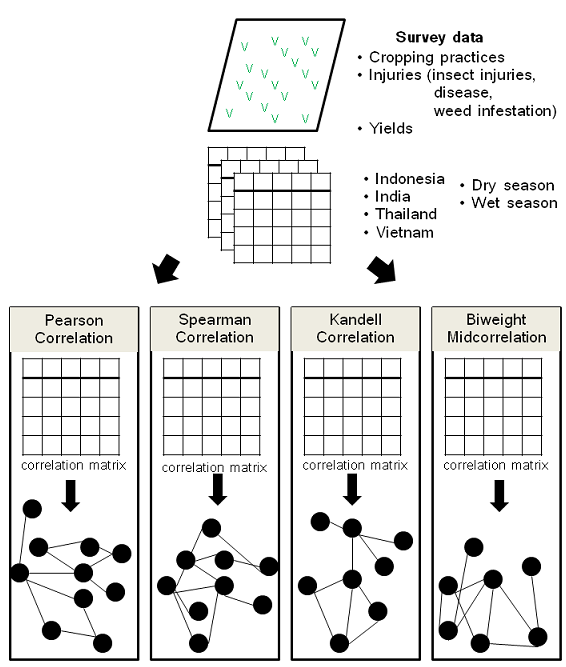
\includegraphics[resolution = 600]{pipeline}
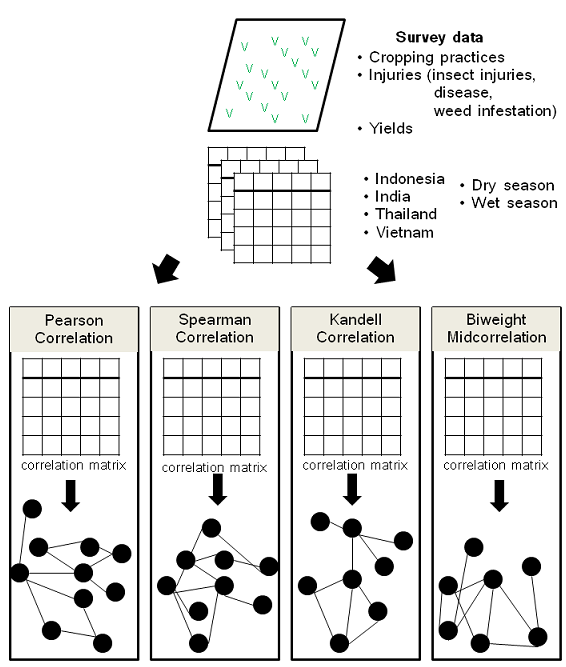
\includegraphics[width = 6in]{pipeline}
\caption[Network method for characterizing interaction between injury profiles and cropping practices using correlation measures]{Crop health surveys data are included cropping practices, injuries, and yield data will collected from different farmers' fields in different countries(Indonesia, India, Thailand, and Vietnam). The correlation matrices will be produced by each individual methods; Pearson, Spearman, Kendall and Biweight midcorrealtion. They will be adjusted $p$~values for all coefficients by FDR correction. The correlation coefficients $p$~values > 0.05 will be removed. Resulting network will be  analyzes for structural properties and infer biological meanings. This will provide a single cropping practices and injury profiles association network for crop health data.}
\end{figure}
%\end{landscape}

\newpage
\begin{landscape}
\begin{figure}
\centering
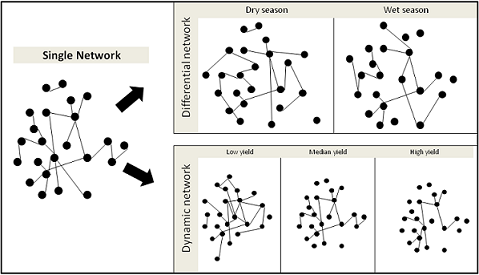
\includegraphics[width=9in]{wholenet}
\caption[Network comparison]{Single network will be created from whole survey data set. Differential network will be constructed using different data set, which may be different seasons (\textit{e.g.}, dry season and wet season) or different geographic locations, then will be measured differences in connectivity patterns between to networks. Dynamic networks will be produced from different data sets with consecutive yield levels, \textit{i.e.}, low, median, high yield.}
\end{figure}
\end{landscape}

%================eos================================
